\documentclass[a4paper,12pt]{article}

\usepackage{graphicx} % Required for inserting images
\usepackage{amsmath,amssymb,amsfonts}
\usepackage{subcaption}
% -----------------------
% Package Imports
% -----------------------

% Set page margins
\usepackage[a4paper, top=1in, bottom=0.8in, left=1.1in, right=0.8in]{geometry}

% Use Times New Roman font
\usepackage{times}

% Add page numbering
\pagestyle{plain}
\usepackage{multirow}
% Enable graphics inclusion
\usepackage{graphicx}
\usepackage{float}
% Enable code listings
\usepackage{listings}
\usepackage{xcolor} % For customizing code colors

% Define MATLAB style for listings
\lstdefinestyle{vscode-light}{
	language=Matlab,
	basicstyle=\ttfamily\footnotesize,
	keywordstyle=\color{blue},
	commentstyle=\color{gray},
	stringstyle=\color{red},
	numberstyle=\tiny\color{black},
	numbersep=5pt,
	frame=single,
	backgroundcolor=\color{white!10},
	breaklines=true,
	captionpos=b,
	tabsize=4,
	showstringspaces=false,
	numbers=left,  % Enable line numbering on the left
	stepnumber=1,  % Line numbers increment by 1
	numberfirstline=true, % Number the first line
}
\setlength{\parindent}{0pt}
\usepackage{sectsty}
\sectionfont{\fontsize{12}{15}\selectfont}

\begin{document}
\section*{Experiment No. 1}

\section*{Experiment Title }
Design, Soldering and Testing of an Astable Multivibrator Circuit Using a 555 Timer
	\section{Objective}

The objectives of this lab are:
\begin{itemize}
\item To study the operation and observe the wave forms of Astable Multivibrator.
\item To Design an Astable Multivibrator PCB board and to generate a square wave.

	
\end{itemize}
\section{Theory}

A Printed Circuit Board (PCB) is a rigid structure that contains electrical circuitry made up of embedded metal. The astable circuit is an oscillator that has two quasi-stable states. It is also called a \textbf{free running multivibrator} and is used to generate a ``Square Wave''. The astable configuration will make successive transitions from one quasi-stable state to the other without an external triggering signal. This allows for fast switching.

In the \textbf{555 Oscillator} circuit, pin 2 and pin 6 are connected together, allowing the circuit to re trigger itself on each and every cycle, enabling it to operate as a free-running oscillator.

During each cycle, the capacitor $C$ charges up through both timing resistors $R_1$ and $R_2$ but discharges only through resistor $R_2$, as the other side of $R_2$ is connected to the discharge terminal, pin 7.

The capacitor charges up to $\frac{2}{3}V_{cc}$ (the upper comparator limit), which is determined by the combination:
\[
0.693(R_1 + R_2)C
\]
and discharges down to $\frac{1}{3}V_{cc}$ (the lower comparator limit), which is determined by:
\[
0.693(R_2 \cdot C)
\]

This results in an output whose ``ON'' and ``OFF'' time periods are determined by the capacitor and resistor combinations.

When connected as an astable multivibrator, the output from the 555 oscillator will continue indefinitely, charging and discharging between $\frac{2}{3}V_{cc}$ and $\frac{1}{3}V_{cc}$, until the power supply is removed.

As with the monostable multivibrator, these charge and discharge times—and therefore the frequency—are independent of the supply voltage.

\section{Circuit Diagram}
	\begin{figure}[H]
	\centering
	\includegraphics[width=1\linewidth]{"Images/1"}
	\caption{Schematic Diagram}
\end{figure}
\section{Required Apparatus}
\begin{table}[H]
	\centering
	\caption{Components list for Astable Multivibrator}
	\begin{tabular}{|c|c|c|c|}
		\hline
		\textbf{\begin{tabular}[c]{@{}c@{}}SI \\ No.\end{tabular}} & \textbf{Components}                                                                   & \textbf{Specifications}                                                                     & \textbf{Quantity} \\ \hline
		1                                                          & PCB board                                                                             & \begin{tabular}[c]{@{}c@{}}Printed connection of\\    \\ astable multivibrator\end{tabular} & 1                 \\ \hline
		2                                                          & Resistor                                                                              & 100k$\Omega$  X 1, 10k$\Omega$ X 1,                               & 2                 \\ \hline
		3                                                          & Capacitor                                                                             & \begin{tabular}[c]{@{}c@{}}1 X 10µF polar , \\    1 X 10nF non polar\end{tabular}           & 2                 \\ \hline
		4                                                          & LED                                                                                   &                                                                                             & 1                 \\ \hline
		5                                                          & Potentiometer                                                                         & 100k$\Omega$                                                                                       & 1                 \\ \hline
		6                                                          & 555 timer with connector                                                              & Model : NE555N                                                                              & 1                 \\ \hline
		7                                                          & DC supply                                                                             & 9V                                                                                          & 1                 \\ \hline
		8                                                          & Jumper wires                                                                          & Male to  Male wire                                                                          & 4                 \\ \hline
		9                                                          & \begin{tabular}[c]{@{}c@{}}Simulating and pcb\\    designing software\end{tabular} & Eagle                                                                                       &                   \\ \hline
	\end{tabular}
\end{table}
\newpage
\section{Experimental Procedure}

\begin{enumerate}
	\item Collected all necessary components including the 555 timer IC, resistors, capacitors, LEDs, power supply, and PCB or vero board.
	\item Referred to the circuit diagram of the astable multivibrator using a 555 timer and placed the components on the board accordingly.
	\item Soldered the components carefully, ensuring correct polarity for the IC, capacitors, and LEDs.
	\item Trimmed excess leads after soldering to prevent short circuits.
	\item Visually inspected the circuit and checked continuity using a multimeter to confirm correct connections.
	\item Connected the power supply (typically 5V or 9V DC) to the circuit.
	\item Observed the LEDs connected at the output pins — they should blink alternately, indicating proper operation.
	\item Optionally, measured the output frequency using an oscilloscope or multimeter to compare with theoretical values.
\end{enumerate}
\section{PCB Design}
	\begin{figure}[H]
	\centering
	\includegraphics[width=0.51\linewidth]{"Images/2"}
	\caption{Schematic Diagram}
\end{figure}
\section{Circuit diagram after soldering}
	\begin{figure}[H]
	\centering
		\begin{subfigure}[t]{1\textwidth}
		\centering
		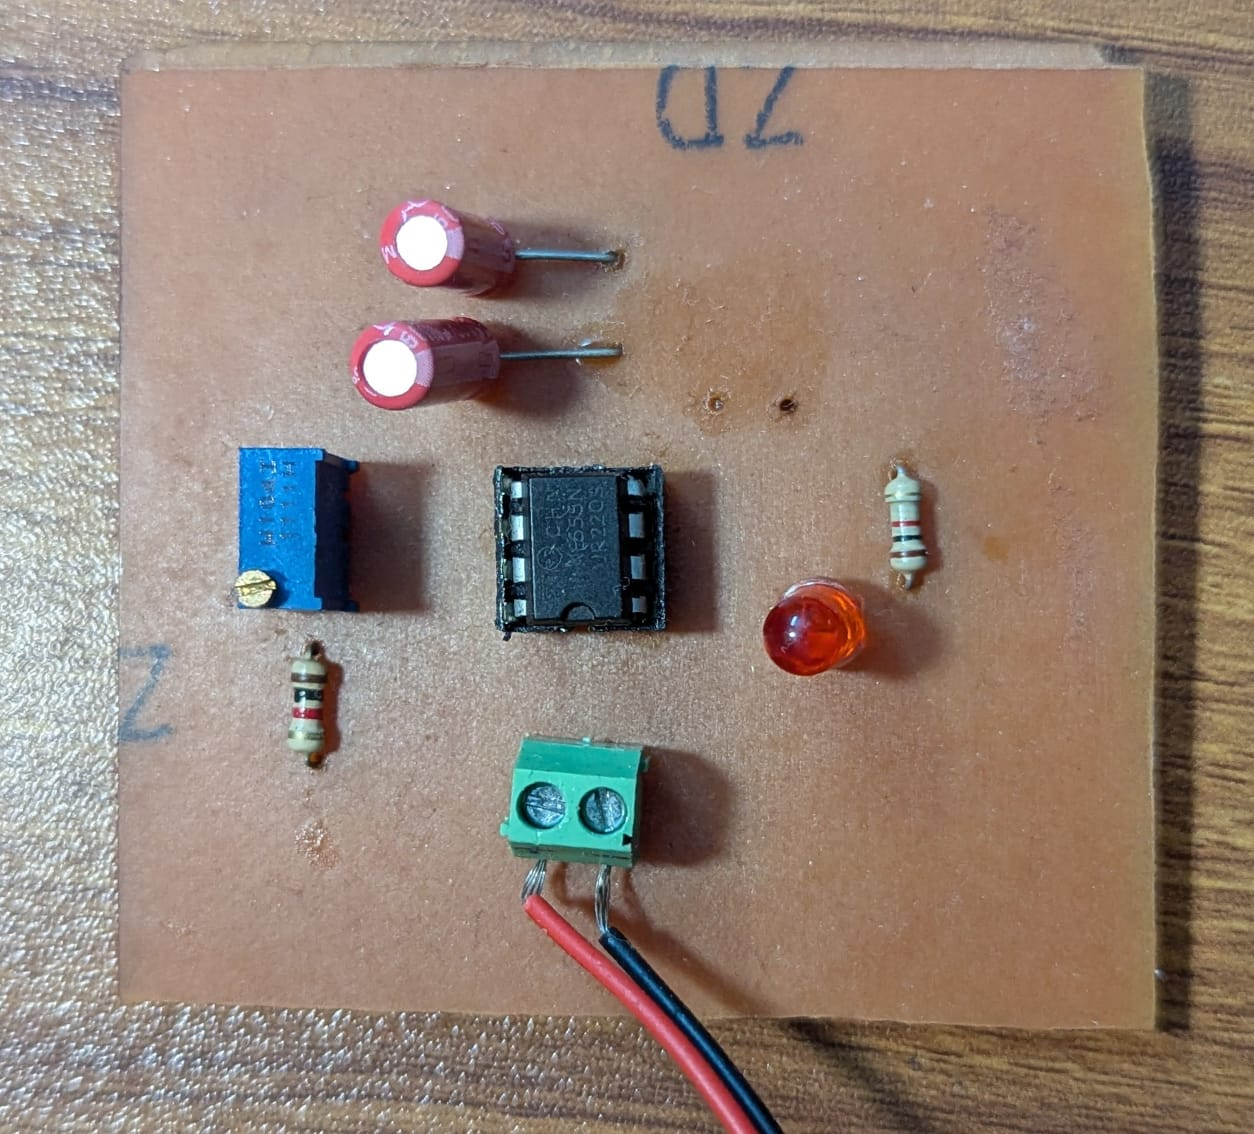
\includegraphics[width=0.5\linewidth]{Images/4}
		\caption{ Top side of the PCB board}
		\vspace{2cm}
	\end{subfigure}
	
	\begin{subfigure}[t]{1\textwidth}
		\centering
		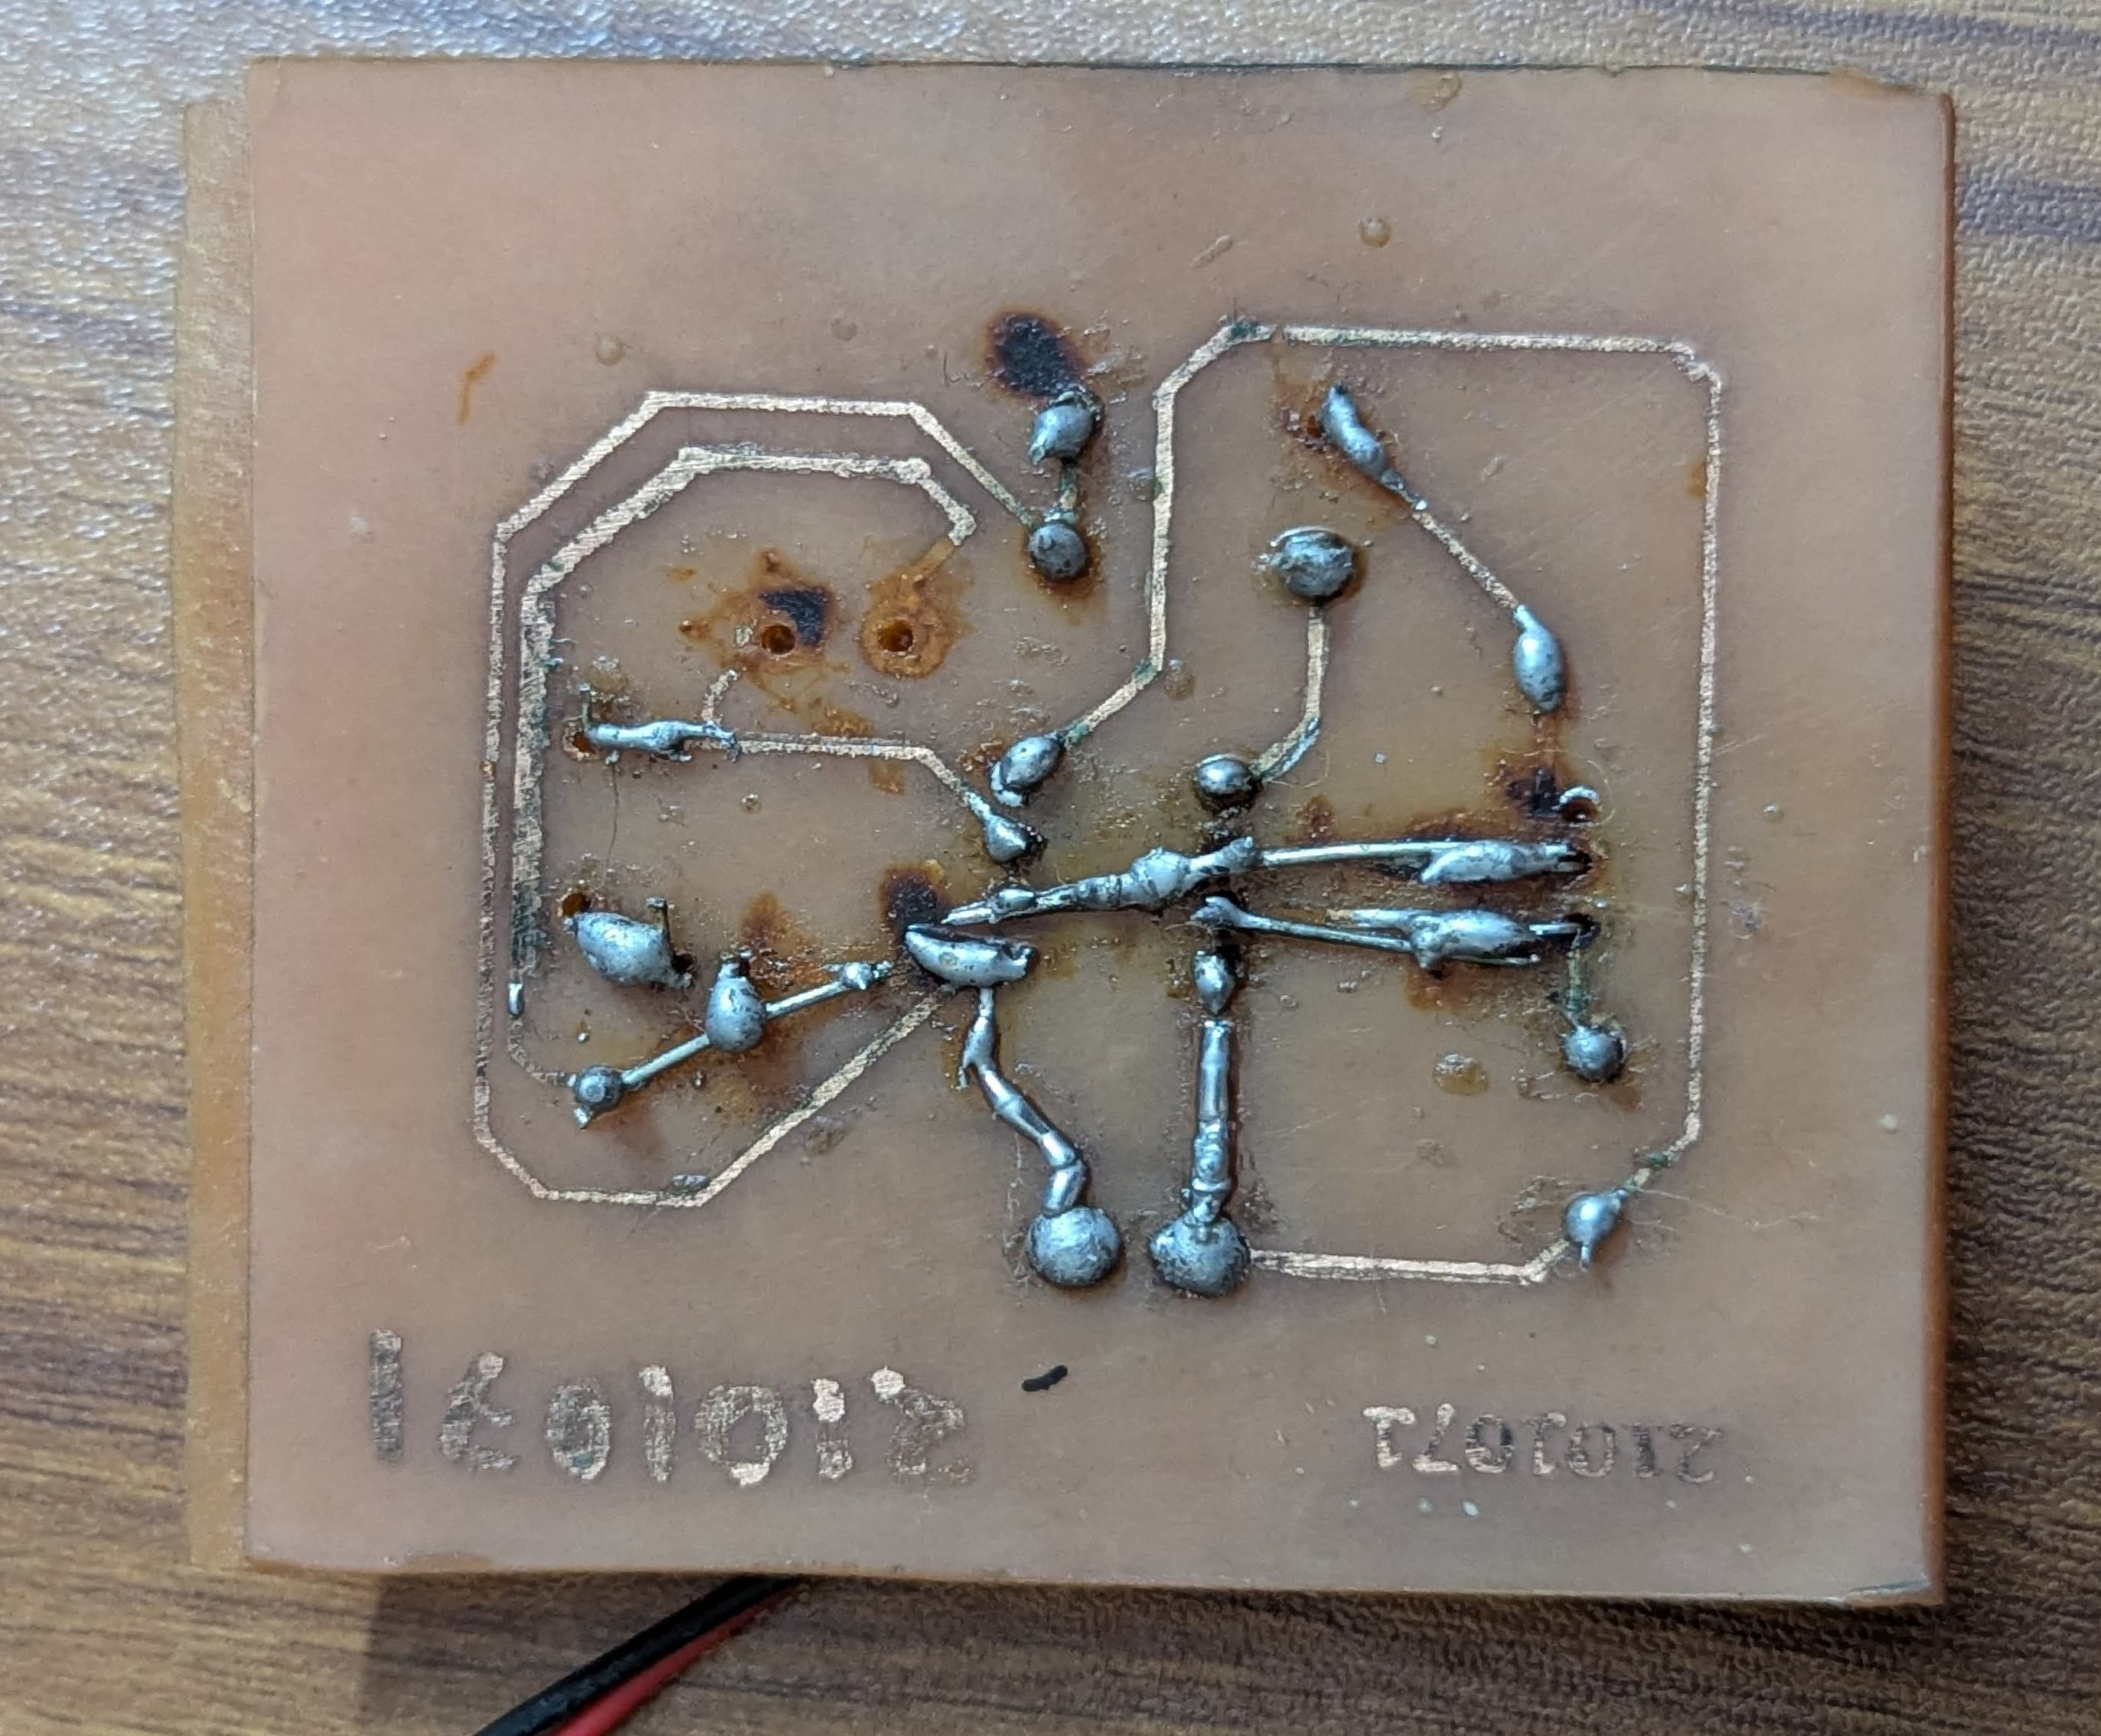
\includegraphics[width=0.5\linewidth]{Images/3}
		\caption{ Bottom side of the PCB board}
	\end{subfigure}
\end{figure}


\section{Theoretical Calculations}

For the full value of the potentiometer:
\begin{enumerate}
	\item \textbf{ On Time} (\( t_1 \))
	\[
	t_1 = 0.693(R_1 + R_2) \times C
	\]
	\[
	t_1 = 0.693(10 + 100) \times 10^3 \times 10 \times 10^{-6}
	\]
	\[
	t_1 = 0.7623 \ \text{seconds}
	\]
	\item \textbf{Off Time} (\( t_2 \))
	\[
	t_2 = 0.693 \times R_2 \times C
	\]
	\[
	t_2 = 0.693 \times 100 \times 10^3 \times 10 \times 10^{-6}
	\]
	\[
	t_2 = 0.693 \ \text{seconds}
	\]
	\item \textbf{Time Period} (\( T \))
	\[
	T = t_1 + t_2
	\]
	\[
	T = 0.7623 + 0.693 = 1.4553 \ \text{seconds}
	\]
	
	\item \textbf{Duty Cycle}
	
	\[
	\text{Duty Cycle} = \frac{\text{On time}}{\text{Time period}} \times 100\%
	\]
	\[
	\text{Duty Cycle} = \frac{0.7623}{1.4553} \times 100\% = 52.38\%
	\]
	
\end{enumerate}



\section{Discussion}
In the shop practice, we were given the task to design, solder, and test an astable multivibrator circuit using a 555 timer IC. But only the designing and soldering of the PCB were done, as the testing of the PCB failed. To make the PCB board, the etching process was followed, where the PCB board was submerged in ferric chloride solution to make the desired tracing path. To place the components, holes were drilled. The components were placed and soldered onto the PCB with great care. To supply the board, a 9V battery was used, which was connected to a screw connector. For a power indicator, an LED was placed to ensure the PCB's power supply, which worked fine as power was supplied.
\section{Conclusion}

 Although the power supply was successfully connected and worked the power LED indicator, the circuit did not work as expected. The possible reasons for the PCB not working could be incorrect component placement, faulty or loose solder joints, damaged components during soldering.As there was no broken or shorted path, we can conclude that damaged components before or during soldering might be the possible and logical reason for unexpected result.


\end{document}